\hypertarget{tiempo-hasta-la-primera-respuesta}{%
\section{Tiempo hasta la primera
respuesta}\label{tiempo-hasta-la-primera-respuesta}}

Pregunta: ¿Cuánto tiempo pasa entre que se crea una actividad que
requiere atención y la primera respuesta?

\hypertarget{descripciuxf3n}{%
\subsection{Descripción}\label{descripciuxf3n}}

La primera respuesta a una actividad a veces puede ser la respuesta más
importante. La primera respuesta muestra que una comunidad es activa y
participa en conversaciones. Un tiempo prolongado para responder a una
actividad puede ser una señal de que una comunidad no es reactiva. Un
breve período de tiempo para responder a una actividad puede ayudar a
involucrar a más miembros en más discusiones y dentro de la comunidad.

\hypertarget{objetivos}{%
\subsection{Objetivos}\label{objetivos}}

Identificar la cadencia de la primera respuesta a través de una variedad
de actividades, incluidas PRs, incidencias, correos electrónicos,
publicaciones de IRC, etc. El tiempo hasta la primera respuesta es una
consideración importante para los contribuyentes nuevos y antiguos a un
proyecto junto con el estado general del proyecto.

\hypertarget{implementaciuxf3n}{%
\subsection{Implementación}\label{implementaciuxf3n}}

Tiempo hasta la primera respuesta de una actividad = hora en que se
publicó la primera respuesta a la actividad - hora en que se creó la
actividad.

\hypertarget{filtros}{%
\subsubsection{Filtros}\label{filtros}}

\begin{itemize}
\tightlist
\item
  Función del respondedor, p. ej., solo se cuentan las respuestas de
  mantenedores
\item
  Respuestas automatizadas, por ejemplo, solo se cuentan las respuestas
  de personas reales mediante el filtrado de bots y otras respuestas
  automatizadas
\item
  Tipo de actividad, p. ej., incidencias (consulte la métrica
  \href{https://github.com/chaoss/wg-evolution/blob/master/metrics/Issue_Response_Time.md}{Tiempo
  de respuesta ante incidencias}), correos electrónicos, chat,
  revisiones de códigos
\end{itemize}

\hypertarget{visualizaciones}{%
\subsubsection{Visualizaciones}\label{visualizaciones}}

\hypertarget{panel-de-grimoirelab-descripciuxf3n-general-del-tiempo-de-eficiencia}{%
\subsection{\texorpdfstring{\protect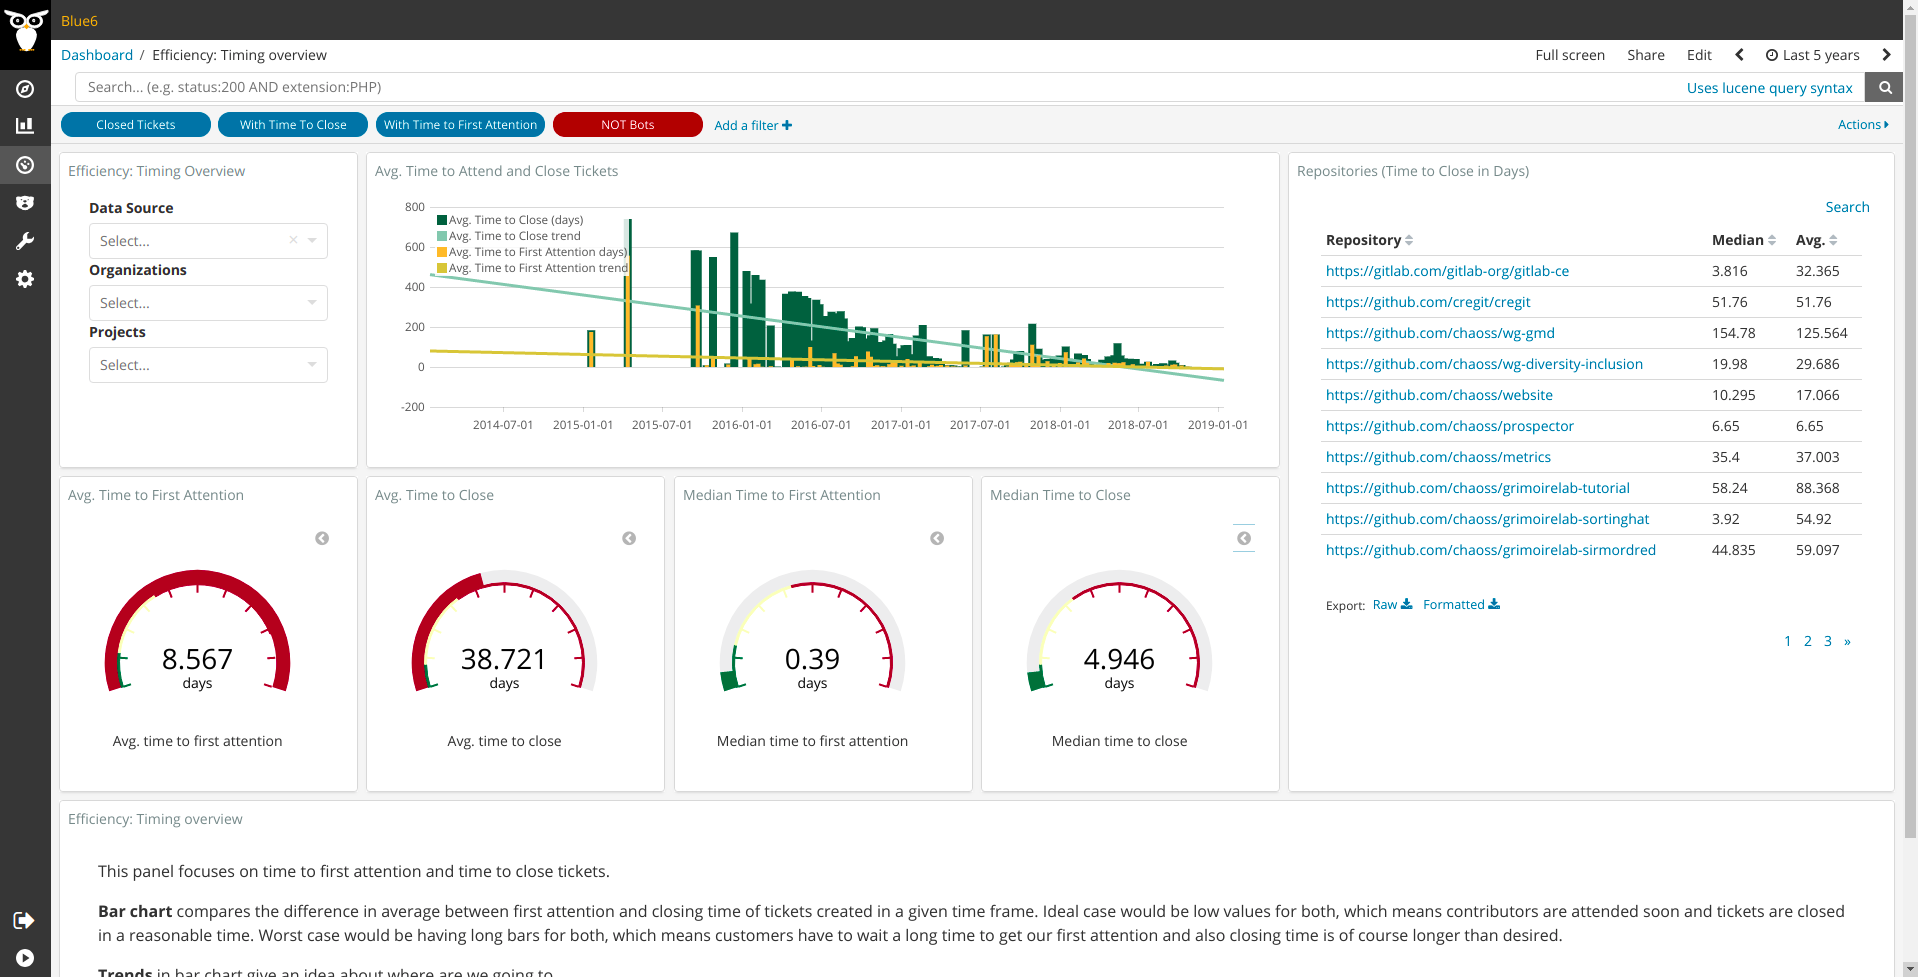
\includegraphics{images/time-to-first-response_efficiency-timing-overview.png}}{Panel de GrimoireLab: descripción general del tiempo de eficiencia}}\label{panel-de-grimoirelab-descripciuxf3n-general-del-tiempo-de-eficiencia}}

\hypertarget{visualizaciuxf3n-de-augur-mapa-de-calor-de-tiempo-hasta-la-primera-respuesta}{%
\subsection{\texorpdfstring{\protect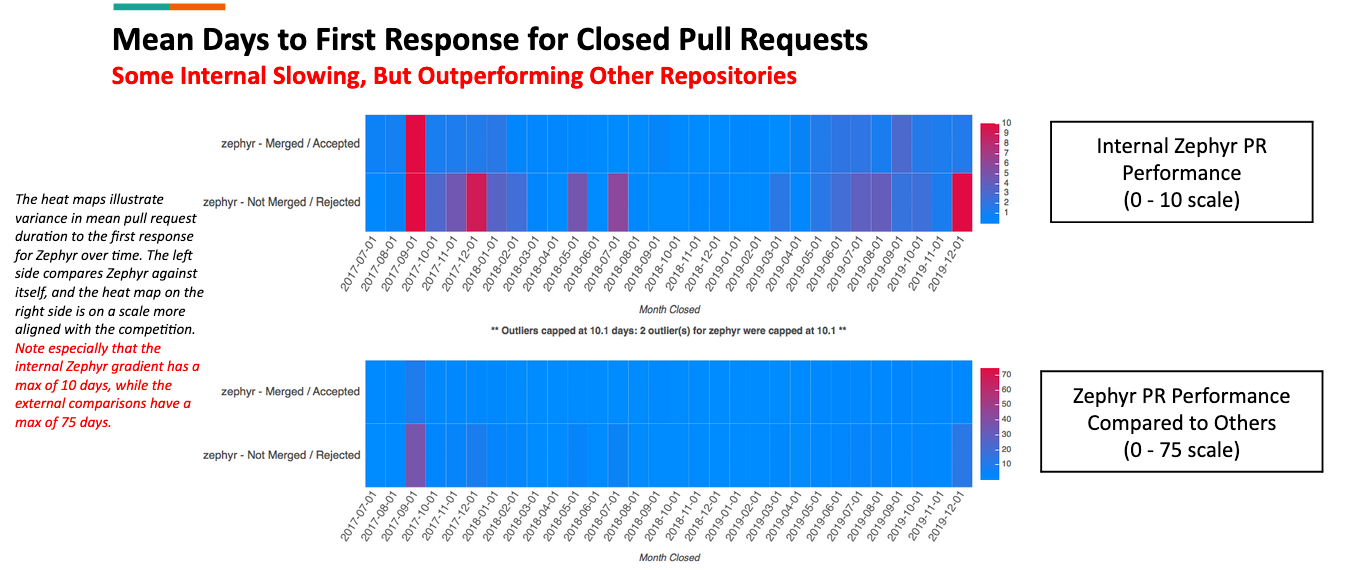
\includegraphics{images/time-to-first-response_augur-ttc-1.png}}{Visualización de Augur: mapa de calor de tiempo hasta la primera respuesta}}\label{visualizaciuxf3n-de-augur-mapa-de-calor-de-tiempo-hasta-la-primera-respuesta}}

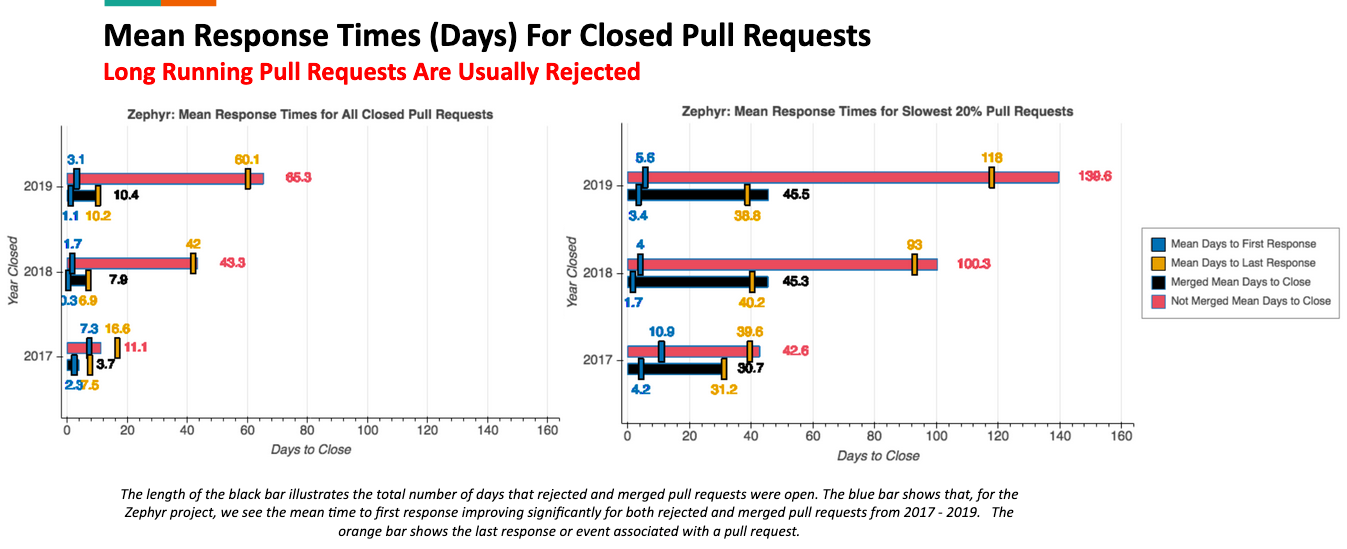
\includegraphics{images/time-to-first-response_augur-ttc-2.png}

\hypertarget{herramientas-que-proporcionan-la-muxe9trica}{%
\subsubsection{Herramientas que proporcionan la
métrica}\label{herramientas-que-proporcionan-la-muxe9trica}}

\begin{itemize}
\tightlist
\item
  Panel de GrimoireLab:
  \href{https://chaoss.github.io/grimoirelab-sigils/panels/efficiency-timing-overview/}{Descripción
  general del tiempo de eficiencia}
\item
  \href{https://katacontainers.biterg.io/app/kibana\#/dashboard/cbbdd920-288c-11e9-b662-975152e57997}{Panel
  de eficiencia del tablero de Kata Containers}
\end{itemize}

\hypertarget{referencias}{%
\subsection{Referencias}\label{referencias}}
